% bod_model.tex - Break-over diode (BOD): device, application circuits and
% Simscape model dtt.crowbar.bod
% Rev. 00, 2026-09-22
% Compile: pdflatex --shell-escape bod_model.tex (twice)
\documentclass[11pt,a4paper]{article}
\usepackage[T1]{fontenc}
\usepackage[utf8]{inputenc}
\usepackage[margin=22mm]{geometry}
\usepackage{amsmath,amssymb}
\usepackage{graphicx}
\usepackage{booktabs}
\usepackage{array}
\usepackage{siunitx}
\usepackage{xcolor}
\usepackage{tikz}
\usetikzlibrary{arrows.meta,positioning,calc,shapes.geometric}
\usepackage{circuitikz}
\ctikzset{voltage dir=EF}
\ctikzset{bipoles/length=1.1cm}
\usepackage{listings}
\usepackage{caption}
\usepackage{fancyhdr}
\setlength{\headheight}{14pt}
\usepackage[hidelinks]{hyperref}

\sisetup{per-mode=symbol,range-phrase=--,range-units=single}
\graphicspath{{fig/}}

\newcommand{\docrev}{Rev.~00}
\newcommand{\docdate}{2026-09-22}
\newcommand{\Vbo}{V_{\mathrm{BO}}}
\newcommand{\Ibo}{I_{\mathrm{BO}}}
\newcommand{\Ih}{I_{\mathrm{H}}}
\newcommand{\Vh}{V_{\mathrm{H}}}
\newcommand{\Vto}{V_{\mathrm{T0}}}
\newcommand{\rT}{r_{\mathrm{T}}}
\newcommand{\Vdrm}{V_{\mathrm{DRM}}}
\newcommand{\Tj}{T_{\mathrm{j}}}
\newcommand{\dvdt}{\mathrm{d}v/\mathrm{d}t}
\newcommand{\ssc}[1]{\texttt{#1}}

\lstset{
  basicstyle=\ttfamily\footnotesize,
  columns=fullflexible,
  keepspaces=true,
  breaklines=true,
  frame=single,
  framerule=0.3pt,
  numbers=left,
  numberstyle=\tiny\color{gray},
  numbersep=6pt,
  commentstyle=\color{black!60},
  showstringspaces=false,
  xleftmargin=1.5em,
}

\pagestyle{fancy}
\fancyhf{}
\lhead{Break-over diode: device, application and Simscape model}
\rhead{\docrev\ -- \docdate}
\cfoot{\thepage}

\title{Break-over diode (BOD): device, application circuits and Simscape model \ssc{dtt.crowbar.bod}\\[4pt]
{\large \docrev\ -- \docdate}}
\author{D. Bagnara}
\date{\docdate}

\begin{document}
\maketitle

\begin{table}[h]
\centering
\caption{Revision history}
\begin{tabular}{@{}llp{9cm}@{}}
\toprule
Rev. & Date & Description \\
\midrule
00 & \docdate & First issue: device description, application circuits, functional Simscape model with switching dynamics and optional thermal port, verification with a Python replica of the model equations. Default data IXBOD2-11. \\
\bottomrule
\end{tabular}
\end{table}

\tableofcontents

%======================================================================
\section{Scope}
This note describes the break-over diode (BOD), the two-terminal p-n-p-n device used as a passive overvoltage trigger for thyristors, and documents the Simscape component \ssc{dtt.crowbar.bod} written for the DTT DIV crowbar models. The component is a functional model (piecewise-linear characteristics, event-based mode switching) with the dynamics that matter for a trigger device: turn-on time, $\dvdt$ triggering, holding-current turn-off and a surrogate of the turn-off time $t_q$. Temperature dependence of the breakover voltage, holding current, off-state current and critical $\dvdt$ is included, with an optional thermal port.

The model equations were verified with a Python replica of the component (\ssc{bod\_sim.py}), which also produced the figures of Section~\ref{sec:verification}. The \ssc{.ssc} file itself has not yet been compiled in MATLAB and must be checked with \ssc{ssc\_build}. The default parameters are those of the Littelfuse/IXYS IXBOD2-11 (\SI{1100}{V} $\pm$ \SI{50}{V}), the device foreseen as backup trigger in the DTT crowbar. Parameters not given in the datasheet are marked as assumed.

%======================================================================
\section{The break-over diode}

\subsection{Structure and operation}
A BOD is a four-layer p-n-p-n silicon device with two terminals, anode (A) and cathode (K), i.e.\ a thyristor without gate (a Shockley diode) engineered so that its forward breakover voltage $\Vbo$ is accurate, stable and reproducible. Figure~\ref{fig:bod_structure} shows the symbol, the layer sequence and the two-transistor equivalent. In forward blocking (anode positive) the outer junctions J1 and J3 are forward biased and the central junction J2 blocks. The leakage current of J2, multiplied by the avalanche factor $M(v)$ of that junction, feeds the bases of the p-n-p and n-p-n transistors; the device switches to the on-state when the loop gain reaches unity,
\begin{equation}
M(v)\,\bigl[\alpha_{1}(i)+\alpha_{2}(i)\bigr] = 1 .
\label{eq:breakover}
\end{equation}
In a thyristor this condition is normally reached by injecting gate current (which raises $\alpha_2$); in a BOD it is reached by the avalanche multiplication $M(v)$ of J2 alone. The breakover voltage is therefore fixed by the avalanche breakdown of J2, which depends on doping and thickness of the n$^-$ base and is well controlled by the process; commercial devices are specified with $\pm$\SI{50}{V} on $\Vbo$ and a positive temperature coefficient of the order of \SIrange{0.7e-3}{2e-3}{\per\kelvin} \cite{ixbod2,ixbod1}. Cathode shorts and guard rings shape the current path so that breakover starts uniformly and the device can withstand the high initial $\mathrm{d}i/\mathrm{d}t$ of a trigger pulse \cite{ixyspatent}.

Two properties distinguish a BOD from a thyristor. First, the small die (a trigger device: \SI{0.9}{A} average, \SI{200}{A} surge for \SI{0.1}{ms} \cite{ixbod2}) gives a fast turn-on: the anode voltage collapses within \SIrange{0.3}{0.5}{\micro\second} of reaching $\Vbo$ \cite{ixyspatent}. Second, the reverse blocking capability is very low: the emitter junctions are heavily doped and shorted, so a discrete BOD element blocks only about \SI{10}{V} in reverse \cite{ixysapp}; whenever the application applies reverse voltage, a series diode is mandatory.

\begin{figure}[htb]
\centering
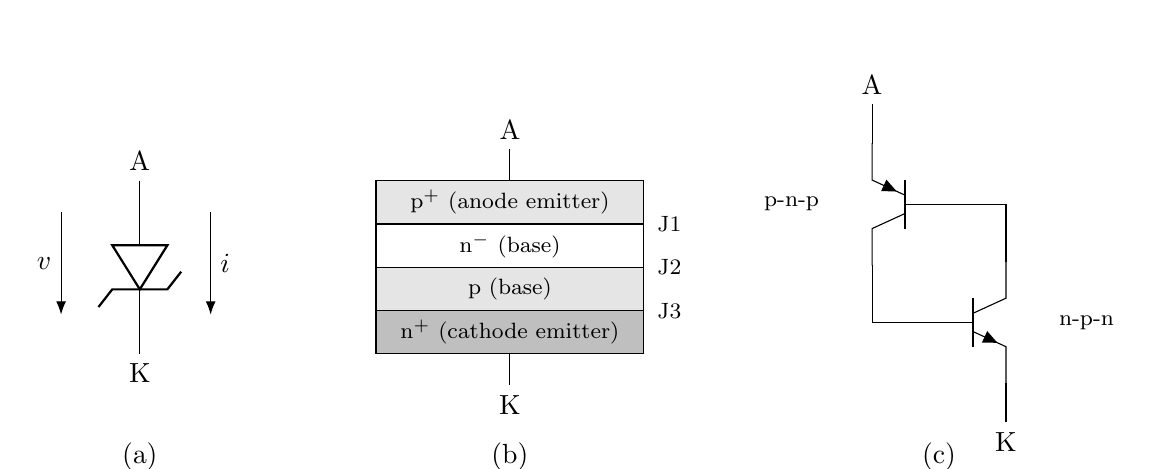
\begin{tikzpicture}[scale=1, >=Latex]
% (a) symbol
\begin{scope}[shift={(0,0)}]
\draw (0,2.2) to[zzD, name=B] (0,0);
\node[above] at (0,2.2) {A};
\node[below] at (0,0) {K};
\draw[->] (-1.0,1.8) -- (-1.0,0.5) node[midway,left]{$v$};
\draw[->] (0.9,1.8) -- (0.9,0.5) node[midway,right]{$i$};
\node at (0,-1.3) {(a)};
\end{scope}
% (b) four-layer structure
\begin{scope}[shift={(3.0,0)}]
\foreach \y/\l/\c in {1.65/p$^{+}$ (anode emitter)/black!10, 1.1/n$^{-}$ (base)/white, 0.55/p (base)/black!10, 0/n$^{+}$ (cathode emitter)/black!25}
  {\draw[fill=\c] (0,\y) rectangle (3.4,\y+0.55); \node at (1.7,\y+0.275) {\footnotesize \l};}
\node[right] at (3.45,1.65) {\footnotesize J1};
\node[right] at (3.45,1.1) {\footnotesize J2};
\node[right] at (3.45,0.55) {\footnotesize J3};
\draw (1.7,2.2) -- (1.7,2.6) node[above]{A};
\draw (1.7,0) -- (1.7,-0.4) node[below]{K};
\node at (1.7,-1.3) {(b)};
\end{scope}
% (c) two-transistor equivalent
\begin{scope}[shift={(9.3,0.3)}]
\node[pnp, xscale=-1] (Q1) at (0,1.6) {};
\node[npn] (Q2) at (1.7,0.1) {};
\draw (Q1.E) -- ++(0,0.5) node[above]{A};
\draw (Q2.E) -- ++(0,-0.5) node[below]{K};
\draw (Q1.C) |- (Q2.B);
\draw (Q2.C) |- (Q1.B);
\node[left, font=\footnotesize] at (-0.55,1.6) {p-n-p};
\node[right, font=\footnotesize] at (2.25,0.1) {n-p-n};
\node at (0.85,-1.6) {(c)};
\end{scope}
\end{tikzpicture}
\caption{Break-over diode: (a) symbol used in this note (two-terminal breakover symbol), (b) four-layer structure, (c) two-transistor equivalent. Breakover occurs when the avalanche multiplication of J2 (the collector junction common to both transistors) makes the loop gain reach unity, Eq.~(\ref{eq:breakover}).}
\label{fig:bod_structure}
\end{figure}

\subsection{Static characteristic}
The static $i$--$v$ characteristic (Fig.~\ref{fig:iv_sketch}) has the S-shape of all p-n-p-n devices: it is single-valued in current (the voltage is a function of the current) and multi-valued in voltage. Four regions are distinguished.
\begin{itemize}
\item \emph{Forward blocking}, $0<v<\Vbo$: the current is the off-state current $I_D$ (\SI{0.2}{\micro\ampere} at \SI{25}{\celsius}, \SI{200}{\micro\ampere} at \SI{125}{\celsius}, both at $0.8\,\Vbo$ for the IXBOD2), rising steeply near $\Vbo$ because of the avalanche multiplication. The breakover point is $(\Vbo, \Ibo)$ with $\Ibo\le\SI{20}{mA}$.
\item \emph{Negative resistance}, from $(\Vbo,\Ibo)$ to the holding point $(\Vh,\Ih)$: unstable for any source with an impedance lower than the magnitude of the negative slope; the operating point jumps along the load line to the on-state.
\item \emph{On-state}, $i>\Ih$: $v = \Vto + \rT\, i$ with $\Vto\approx\SI{0.9}{V}$, $\rT\approx\SI{80}{m\ohm}$; $V_T=\SI{1.3}{V}$ at \SI{5}{A}. The holding voltage $\Vh$ (\SIrange{4}{8}{V}) is the voltage at $\Ih$, before the full conductivity modulation.
\item \emph{Turn-off} occurs when the current falls below the holding current $\Ih$ (\SI{40}{mA} at \SI{25}{\celsius}, \SI{20}{mA} at \SI{125}{\celsius}); the device then returns to the blocking branch.
\item \emph{Reverse}: blocking up to $V_{RB}\approx\SI{10}{V}$ only, then breakdown of the emitter junctions.
\end{itemize}

\begin{figure}[htb]
\centering
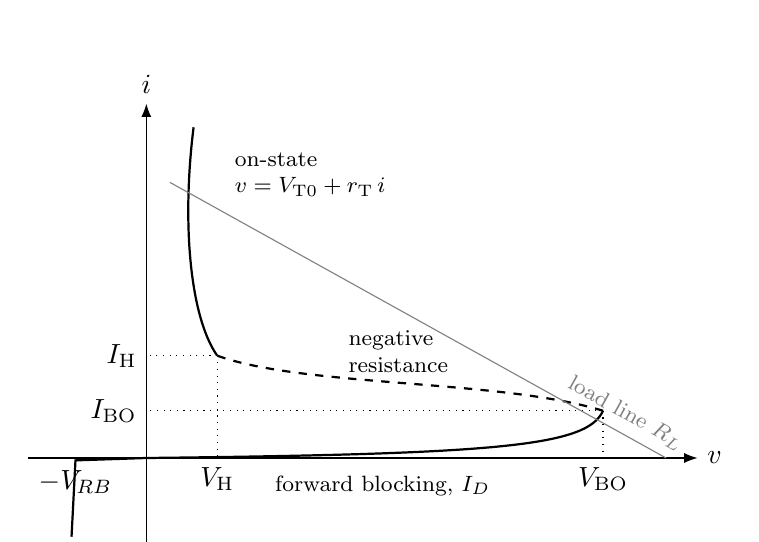
\begin{tikzpicture}[>=Latex, scale=1]
\draw[->] (-1.5,0) -- (7,0) node[right]{$v$};
\draw[->] (0,-1.2) -- (0,4.5) node[above]{$i$};
% blocking branch
\draw[thick] (0,0) .. controls (4.5,0.05) and (5.6,0.15) .. (5.8,0.6);
% negative resistance
\draw[thick, dashed] (5.8,0.6) .. controls (4.5,1.0) and (2.0,0.9) .. (0.9,1.3);
% on-state
\draw[thick] (0.9,1.3) .. controls (0.55,1.8) and (0.45,3.0) .. (0.6,4.2);
% reverse
\draw[thick] (0,0) -- (-0.9,-0.03) -- (-0.95,-1.0);
% markers
\draw[dotted] (5.8,0.6) -- (5.8,0) node[below]{$\Vbo$};
\draw[dotted] (5.8,0.6) -- (0,0.6) node[left]{$\Ibo$};
\draw[dotted] (0.9,1.3) -- (0,1.3) node[left]{$\Ih$};
\draw[dotted] (0.9,1.3) -- (0.9,0) node[below]{$\Vh$};
\node[below] at (-0.9,-0.03) {$-V_{RB}$};
\node[right, align=left, font=\footnotesize] at (1.0,3.6) {on-state\\ $v=\Vto+\rT\,i$};
\node[align=left, font=\footnotesize] at (3.2,1.35) {negative\\ resistance};
\node[font=\footnotesize] at (3.0,-0.35) {forward blocking, $I_D$};
% load line
\draw[gray] (6.6,0) -- (0.3,3.5) node[pos=0.1, above, sloped, font=\footnotesize]{load line $R_L$};
\end{tikzpicture}
\caption{Qualitative static characteristic of a BOD. With a source of open-circuit voltage above $\Vbo$ and series resistance $R_L$ the operating point jumps from $(\Vbo,\Ibo)$ to the on-state along the load line; it jumps back to the blocking branch when the current falls below $\Ih$.}
\label{fig:iv_sketch}
\end{figure}

\subsection{Dynamic characteristics}
\paragraph{Turn-on.} Once $v$ reaches $\Vbo$ the regenerative process of Eq.~(\ref{eq:breakover}) takes a time of the order of the carrier transit time through the n$^-$ base; the datasheets give no figure, the IXYS patent literature quotes a turn-on time (anode voltage collapse) of about \SI{0.5}{\micro\second} for conventional dice and below \SI{0.3}{\micro\second} for the thin epitaxial ones \cite{ixyspatent}. During this time the BOD behaves approximately as a voltage clamp at $\Vbo$: the current is set by the external circuit while the voltage collapses.

\paragraph{$\dvdt$ triggering.} A fast rise of the anode voltage drives the displacement current $C_j\,\dvdt$ of J2 through the bases of the two transistors; if this current, multiplied by $M(v)$, is large enough the device breaks over below $\Vbo$. The datasheet gives a critical rate of \SI{3000}{V\per\micro\second} at $v=0.9\,\Vbo$, \SI{25}{\celsius} (\SI{1000}{V\per\micro\second} at \SI{150}{\celsius} in older revisions) \cite{ixbod2}. The capability is much lower at low voltage because $M(v)$ is small there; conversely, near $\Vbo$ a modest $\dvdt$ is enough. In thyristor protection circuits this is harmless (the BOD only fires the thyristor a little early), but it matters when the BOD stack is exposed to the switching $\dvdt$ of a converter, as happened with the DTT crowbar \cite{crowbardtt}.

\paragraph{$\mathrm{d}i/\mathrm{d}t$ and surge.} The trigger current must be limited by the series resistor: \SI{150}{A\per\micro\second} repetitive, \SI{500}{A\per\micro\second} non-repetitive, $I_{SM}=\SI{200}{A}$ and $I^2t=\SI{4}{A^2 s}$ for \SI{0.1}{ms} \cite{ixbod2}. The junction temperature rise per pulse is estimated with the energy coefficient $K_P=\SI{700}{K\per\joule}$, i.e.\ an adiabatic thermal capacitance of \SI{1.43}{mJ\per\kelvin}.

\paragraph{Turn-off time.} After conduction the stored charge must recombine before the full $\Vbo$ can be blocked again: $t_q=\SI{200}{\micro\second}$ (typical, \SI{150}{\micro\second} for the IXBOD1) \cite{ixbod2,ixbod1}. A forward voltage re-applied earlier re-triggers the device at a lower voltage.

\subsection{Datasheet data of the default device}
Table~\ref{tab:datasheet} collects the IXBOD2-11 data used for the default parameters \cite{ixbod2}, complemented with the IXBOD1 application data \cite{ixysapp}. Where the two datasheet revisions found differ (e.g.\ $\Ibo$ 15 or \SI{20}{mA}, $K_T$ 0.7 or \SI{1e-3}{\per\kelvin}) the values of the current Littelfuse revision were taken.

\begin{table}[htb]
\centering
\caption{IXBOD2-11 data (Littelfuse/IXYS) \cite{ixbod2,ixysapp}}
\label{tab:datasheet}
\footnotesize
\begin{tabular}{@{}llll@{}}
\toprule
Symbol & Quantity & Value & Conditions \\
\midrule
$\Vbo$ & Breakover voltage & \SI{1100 \pm 50}{V} & $\Tj=\SI{25}{\celsius}$ \\
$K_T$ & Temperature coefficient of $\Vbo$ & \SI{1e-3}{\per\kelvin} & \\
$\Ibo$ & Breakover current & \SI{20}{mA} max & $\Tj=\SI{25}{\celsius}$ \\
$I_D$ & Off-state current & \SI{0.2}{\micro\ampere} / \SI{200}{\micro\ampere} max & $0.8\,\Vbo$, 25 / \SI{125}{\celsius} \\
$\Ih$ & Holding current & \SI{40}{mA} / \SI{20}{mA} max & 25 / \SI{125}{\celsius} \\
$\Vh$ & Holding voltage & \SIrange{4}{8}{V} & \SI{25}{\celsius} (IXBOD1 data) \\
$V_T$ & On-state voltage & \SI{1.3}{V} max & $I_T=\SI{5}{A}$, \SI{25}{\celsius} \\
$\Vto$, $\rT$ & Threshold voltage, slope resistance & \SI{0.9}{V}, \SI{80}{m\ohm} & \SI{150}{\celsius} \\
$V_{RB}$ & Reverse blocking voltage & \SI{10}{V} max & IXBOD element \cite{ixysapp} \\
$(\dvdt)_{cr}$ & Critical rate of rise of off-state voltage & \SI{3000}{V\per\micro\second} & $0.9\,\Vbo$, \SI{25}{\celsius} \\
$(\mathrm{d}i/\mathrm{d}t)_{cr}$ & Critical rate of rise of on-state current & 150 / \SI{500}{A\per\micro\second} & repetitive / non-repetitive \\
$t_q$ & Turn-off time & \SI{200}{\micro\second} typ. & \\
$I_{F(AV)M}$, $I_{RMS}$ & Average, RMS current & \SI{0.9}{A}, \SI{1.4}{A} & \SI{50}{Hz}, $T_{amb}=\SI{50}{\celsius}$ \\
$I_{SM}$, $I^2t$ & Surge current, $I^2t$ & \SI{200}{A}, \SI{4}{A^2 s} & $t_p=\SI{0.1}{ms}$ \\
$K_P$ & Energy coefficient & \SI{700}{K\per\joule} & $\Delta\Tj = K_P\,E_{pulse}$ \\
$R_{th(j\text{-}a)}$ & Thermal resistance junction--ambient & 60 / \SI{45}{K\per\watt} & natural / \SI{2}{m/s} air \\
$\Tj$ & Junction temperature range & \SIrange{-40}{150}{\celsius} & \\
\bottomrule
\end{tabular}
\end{table}

%======================================================================
\section{Application: overvoltage protection and self-firing of thyristors}
\label{sec:application}

\subsection{Principle}
Figure~\ref{fig:protection} shows the classical BOD protection circuit \cite{lawatsch1988,ixysapp}. The BOD is connected between the anode and the gate of the thyristor T through the current-limiting resistor $R_1$ and the series diode $D_1$; the gate network $R_2 \parallel C_2$ and the gate lead to the gate unit are the usual ones. When the anode--cathode voltage reaches $\Vbo$ (plus the small drops on $D_1$ and on the gate), the BOD breaks over and a gate current $i_G \approx (v_{AK}-V_T)/R_1$ flows: the thyristor turns on after its gate-controlled delay time $t_{gd}$, the anode voltage collapses and the BOD current falls below $\Ih$, so that the BOD turns off by itself. The thyristor is thus fired \emph{before} its own breakover voltage is reached, in a controlled way through the gate rather than through the uncontrolled bulk breakover, which would concentrate the current in a small area and destroy the device. The same circuit serves as the passive self-firing network of a crowbar: the BOD sets the voltage at which the crowbar closes without any electronics.

\begin{figure}[htb]
\centering
\begin{circuitikz}[scale=1.22, transform shape, >=Latex]
% source and line inductance
\draw (0,0) to[battery2, l_=$V_s$, invert] (0,4.6);
\draw (0,4.6) to[L, l=$L_s$] (2.6,4.6) to[short, -*] (4.0,4.6) to[short, -*] (6.0,4.6) node[above]{A};
\draw (0,0) to[short, -*] (4.0,0) to[short, -*] (6.0,0) node[below]{K};
% snubber (left of the thyristor)
\draw (4.0,4.6) to[R, l=$R_s$] (4.0,2.7) to[C, l=$C_s$] (4.0,0);
% thyristor
\draw (6.0,4.6) to[Ty, l=T, name=T] (6.0,0);
\draw[->] (5.2,4.2) -- (5.2,0.4) node[midway, left]{$v_{AK}$};
% BOD branch
\draw (6.0,4.6) to[short] (9.8,4.6) to[D, l=$D_1$] (9.8,3.5) to[zzD, l_=BOD] (9.8,2.2) to[R, l=$R_1$] (9.8,1.1) to[short, -*] (9.8,0.9) node[below right]{G};
\draw[->] (10.9,3.4) -- (10.9,2.3) node[midway, right]{$v_{BOD}$};
% gate connection
\draw (T.G) -| (7.4,0.9) to[short] (9.8,0.9);
\draw[->] (8.2,1.25) -- (9.2,1.25) node[midway, above]{$i_G$};
% gate network
\draw (9.8,0.9) to[short] (11.6,0.9) to[R, l=$R_2$] (11.6,-1.0) to[short] (6.0,-1.0) to[short] (6.0,0);
\draw (11.6,0.9) to[short] (13.0,0.9) to[C, l=$C_2$] (13.0,-1.0) to[short] (11.6,-1.0);
\end{circuitikz}
\caption{BOD overvoltage protection / self-firing of a thyristor: series diode $D_1$ (takes the reverse voltage, the BOD blocks only about \SI{10}{V}), BOD, current-limiting resistor $R_1$ (\SIrange{0}{200}{\ohm}), gate network $R_2\parallel C_2$ (\SIrange{100}{1000}{\ohm}, \SIrange{22}{47}{nF}) against spurious triggering \cite{ixysapp}. $R_s$--$C_s$ is the usual thyristor snubber.}
\label{fig:protection}
\end{figure}

The sequence of events after the anode voltage exceeds $\Vbo$ is: BOD turn-on ($t_d\approx\SI{0.3}{\micro\second}$), rise of the gate current to the level set by $R_1$, thyristor turn-on after $t_{gd}$ (a few \si{\micro\second} for large phase-control thyristors), collapse of $v_{AK}$. During $t_d + t_{gd}$ the anode voltage keeps rising at the rate imposed by the circuit, so the peak voltage seen by the thyristor is
\begin{equation}
V_{pk} \approx \Vbo + \left.\frac{\mathrm{d}v}{\mathrm{d}t}\right|_{\text{circuit}} (t_d + t_{gd}) ,
\label{eq:vpk}
\end{equation}
which must stay below $\Vdrm$ of the thyristor. With the \SI{100}{V\per\micro\second} limit of the DTT pre-filter \cite{crowbardtt} and $t_d+t_{gd}\approx\SI{4}{\micro\second}$ the overshoot is about \SI{400}{V}.

\subsection{Design rules}
\begin{enumerate}
\item \emph{Choice of $\Vbo$.} The BOD must not fire during normal operation and must fire before the thyristor breaks over:
\begin{equation}
V_{op,max} + \Delta V_{margin} \le \Vbo^{min}(\Tj) , \qquad
\Vbo^{max}(\Tj) + \left.\frac{\mathrm{d}v}{\mathrm{d}t}\right|_{\text{circuit}} (t_d+t_{gd}) \le \Vdrm ,
\label{eq:vbo_choice}
\end{equation}
where $\Vbo^{min,max}$ include the $\pm\SI{50}{V}$ tolerance and the temperature coefficient $K_T$ over the operating range ($+\SI{12.5}{\percent}$ at \SI{150}{\celsius} with $K_T=\SI{1e-3}{\per\kelvin}$). In the DTT option-B configuration the shunt regulator level was \SI{920}{V} and the backup BOD \SI{1100}{V} \cite{crowbardtt}: the minimum breakover \SI{1050}{V} at \SI{25}{\celsius} leaves \SI{130}{V} of margin; at \SI{-40}{\celsius} the margin shrinks to about \SI{60}{V}.
\item \emph{Series stacking.} Higher voltages use $n$ elements in series (modules with 2--4 dice are standard): $\Vbo$ and $V_T$ add ($V_T = 1.7\,n$ V for the IXBOD1 modules), the tolerance grows as $n\times\SI{50}{V}$ and the static voltage sharing is provided by parallel resistors $R_p$ across each element, sized so that their current is large compared with the spread of the off-state currents. Series connection increases the $\dvdt$ capability (the junction capacitances are in series) \cite{ixysapp}.
\item \emph{Current-limiting resistor $R_1$.} It sets the gate current and the BOD current: $i_G \approx (\Vbo - V_{GK})/R_1$ must be several times $I_{GT}$ of the thyristor for a fast, safe turn-on but below the peak forward gate current $I_{FGM}$ (\SI{10}{A} for the 5STP\,26N6500 used in the static-switch bench \cite{crowbarself}) and within the BOD surge and $\mathrm{d}i/\mathrm{d}t$ limits. Values of \SIrange{0}{200}{\ohm} are recommended \cite{ixysapp}; \SIrange{100}{150}{\ohm} give \SIrange{7}{11}{A} with an \SI{1100}{V} BOD. $R_1$ also damps the loop formed by the gate capacitance $C_2$ and the lead inductances.
\item \emph{Series diode $D_1$.} It must block the full reverse voltage applied to the thyristor (anode negative), since the BOD withstands only $V_{RB}\approx\SI{10}{V}$, and it must be a fast, soft-recovery diode: at the end of each BOD pulse the reverse recovery of $D_1$ is what drives the BOD into reverse. Its avalanche capability must cover the recovery of the thyristor.
\item \emph{Gate network.} $R_2\parallel C_2$ (\SIrange{100}{1000}{\ohm}, \SIrange{22}{47}{nF}) keeps the gate at low impedance for noise and for the currents injected through the anode--gate capacitances at high $\dvdt$. It does not delay the firing: the gate--cathode junction clamps the gate voltage at about $V_{GT}$, so $C_2$ only has to be charged to a few volts, which a trigger current of several amperes does in tens of nanoseconds (Fig.~\ref{fig:protection_sim}).
\item \emph{Energy and repetition.} The energy per event in the BOD is small: about $\tfrac{1}{2}\Vbo\, i\, t_d$ during the voltage collapse plus $V_T\, i_G\, t_{gd}$ in the on-state, i.e.\ \SIrange{0.2}{0.3}{mJ} at \SI{10}{A} (Section~\ref{sec:verification}), a temperature rise $K_P E$ of a fraction of a kelvin. The energy goes into $R_1$ instead, $E_{R1}\approx \Vbo\, i_G\,(t_d+t_{gd}) \approx \SI{40}{mJ}$ per event at \SI{10}{A}, which requires a pulse-rated resistor. The average dissipation is negligible at the repetition rates of a crowbar, but the junction temperature before the event (ambient, self-heating of the resistors nearby) shifts $\Vbo$ through $K_T$.
\item \emph{Spurious triggering by $\dvdt$.} The BOD sees the anode $\dvdt$ through $D_1$ and the gate network; with the switching edges of an IGBT bridge (\si{kV\per\micro\second}) a stack close to its $\Vbo$ fires even if the voltage stays below $\Vbo$. This is exactly what the DTT crowbar did at the first switch-on \cite{crowbardtt}. The remedies are the pre-filter (limit the $\dvdt$ at the crowbar node), a small $R$--$C$ across the BOD branch, or a larger margin between the operating voltage and $\Vbo$: the criterion of Section~\ref{sec:dvdt_model} shows that the trigger level scales as $0.9\,\Vbo\,(\dvdt)_{cr}/(\dvdt)$.
\end{enumerate}

%======================================================================
\section{The Simscape model \ssc{dtt.crowbar.bod}}
\label{sec:model}

\subsection{Structure and modes}
The component (Fig.~\ref{fig:model_structure}) has the electrical ports \ssc{p} (anode) and \ssc{n} (cathode), the physical-signal output \ssc{M} (mode indicator) and the optional thermal port \ssc{H}. Electrically it is a conduction current $i_{dev}(v,\,\text{mode})$ in parallel with the junction capacitance $C_j$:
\begin{equation}
i = i_{dev} + C_j \frac{\mathrm{d}v}{\mathrm{d}t} .
\end{equation}
The capacitance makes $v$ a state in every mode, which keeps the equation structure identical across modes, provides the $\dvdt$ needed by the $\dvdt$ trigger criterion and gives the device voltage a physical continuity at the mode transitions. The mode chart has four modes:
\begin{itemize}
\item \ssc{Blocking} ($M=0$): forward blocking with off-state current and pre-breakover term, reverse breakdown beyond $-V_{RB}$; the blocking capability $x_b$ recovers towards 1.
\item \ssc{Triggered} ($M=1$) and \ssc{TriggeredDV} ($M=2$): turn-on after a voltage or a $\dvdt$ trigger; the device acts as a clamp at the voltage $v_{cl}(x_b)$, which collapses exponentially from $\Vbo(\Tj)$ to $\Vto$ while $x_b$ decays from 1 to $x_{on}=10^{-3}$ in the time $t_d$.
\item \ssc{On} ($M=3$): on-state $v = \Vto + \rT\, i_{dev}$, left when $i_{dev} < \Ih(\Tj)$.
\end{itemize}
The blocking-capability state $x_b\in[0,1]$ is the single internal state besides $v$: it drives the turn-on collapse (\ssc{Triggered} and \ssc{On}) and the recovery after turn-off (\ssc{Blocking}), and it defines the actual breakover level $V_{blk}(x_b)$ during recovery. No \ssc{delay()} function and no \ssc{initial} section are used, in line with the constraints found in the \ssc{+dtt/+crowbar} package \cite{crowbardtt}: the first declared mode, \ssc{Blocking}, is the initial one.

\begin{figure}[htb]
\centering
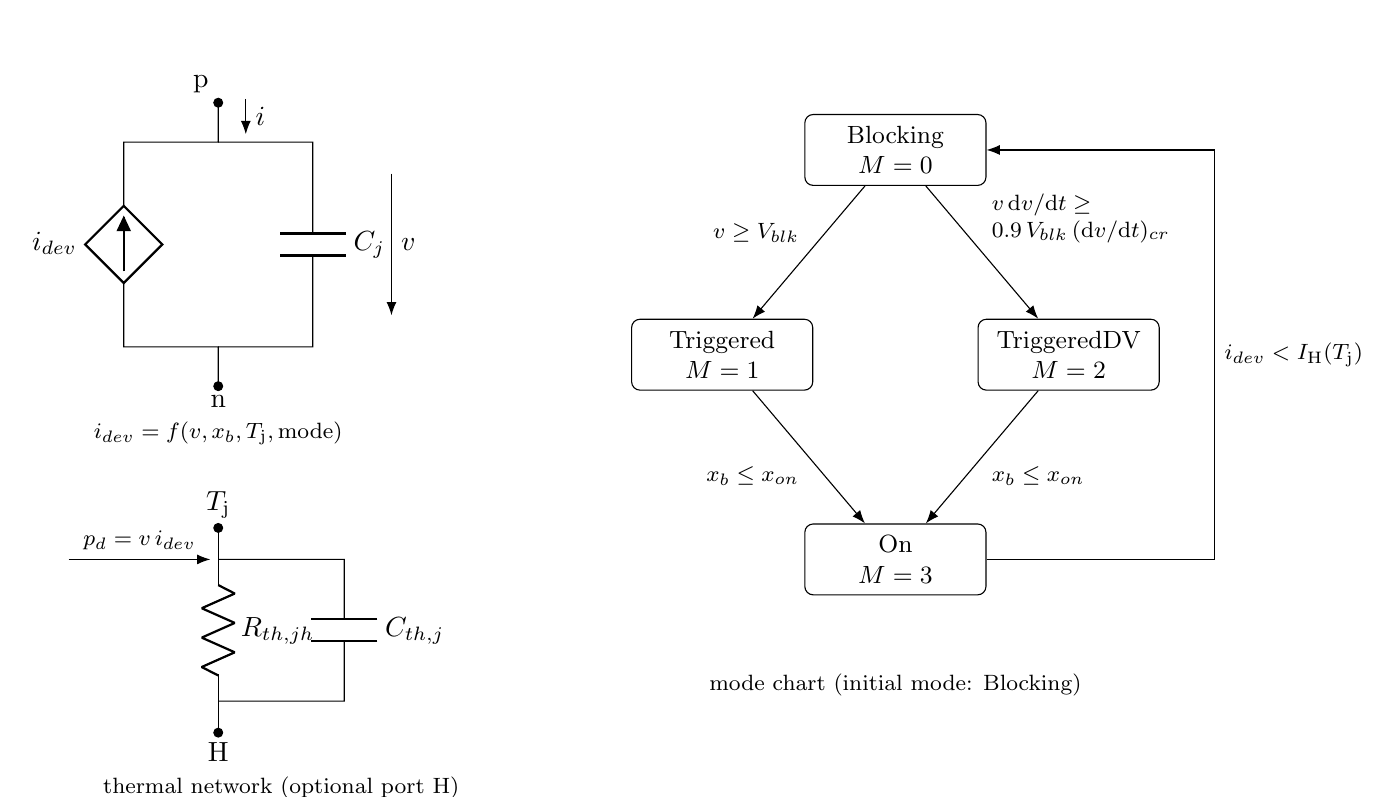
\begin{tikzpicture}[>=Latex,
  mode/.style={draw, rounded corners=3pt, minimum width=2.3cm, minimum height=0.9cm, align=center, font=\small}]
% ---- equivalent circuit (left, top)
\begin{scope}[shift={(0,0)}]
\draw (0,0) node[above left]{p} to[short, *-] (0,-0.5) to[short] (-1.2,-0.5) to[american controlled current source, l_=$i_{dev}$, invert] (-1.2,-3.1) to[short] (0,-3.1) to[short, -*] (0,-3.6) node[below]{n};
\draw (0,-0.5) to[short] (1.2,-0.5) to[C, l=$C_j$] (1.2,-3.1) to[short] (0,-3.1);
\draw[->] (2.2,-0.9) -- (2.2,-2.7) node[midway, right]{$v$};
\draw[->] (0.35,0.05) -- (0.35,-0.4) node[midway, right]{$i$};
\node[align=left, font=\footnotesize] at (0,-4.2) {$i_{dev} = f(v, x_b, \Tj, \text{mode})$};
\end{scope}
% ---- thermal network (left, bottom)
\begin{scope}[shift={(0,-5.4)}]
\draw (0,0) node[above]{$\Tj$} to[short, *-] (0,-0.4) to[R, l=$R_{th,jh}$] (0,-2.2) to[short, -*] (0,-2.6) node[below]{H};
\draw (0,-0.4) to[short] (1.6,-0.4) to[C, l=$C_{th,j}$] (1.6,-2.2) to[short] (0,-2.2);
\draw[->] (-1.9,-0.4) -- (-0.1,-0.4) node[midway, above, font=\footnotesize]{$p_d = v\,i_{dev}$};
\node[font=\footnotesize, align=center] at (0.8,-3.3) {thermal network (optional port H)};
\end{scope}
% ---- mode chart (right)
\begin{scope}[shift={(8.6,0)}]
\node[mode] (B)  at (0,-0.6)  {Blocking\\ $M=0$};
\node[mode] (T)  at (-2.2,-3.2) {Triggered\\ $M=1$};
\node[mode] (TD) at (2.2,-3.2)  {TriggeredDV\\ $M=2$};
\node[mode] (O)  at (0,-5.8)  {On\\ $M=3$};
\draw[->] (B) -- node[midway, above left, font=\footnotesize]{$v\ge V_{blk}$} (T);
\draw[->] (B) -- node[midway, above right, font=\footnotesize, align=left]{$v\,\dvdt \ge$\\ $0.9\,V_{blk}\,(\dvdt)_{cr}$} (TD);
\draw[->] (T) -- node[midway, below left, font=\footnotesize]{$x_b\le x_{on}$} (O);
\draw[->] (TD) -- node[midway, below right, font=\footnotesize]{$x_b\le x_{on}$} (O);
\draw[->] (O.east) -- ++(2.9,0) |- (B.east) node[pos=0.25, right, font=\footnotesize]{$i_{dev}<\Ih(\Tj)$};
\node[font=\footnotesize] at (0,-7.4) {mode chart (initial mode: Blocking)};
\end{scope}
\end{tikzpicture}
\caption{Structure of the model: conduction current $i_{dev}$ in parallel with $C_j$; thermal network between the junction and the port H (only with \ssc{thermal\_port = on}); mode chart with the transition predicates.}
\label{fig:model_structure}
\end{figure}

\subsection{Equations}
\paragraph{Temperature dependence.} With $\Delta T = \Tj - \SI{25}{\celsius}$,
\begin{align}
\Vbo(\Tj) &= \Vbo\,(1 + K_T\,\Delta T) , \label{eq:vbot}\\
\Ih(\Tj)  &= \Ih^{25}\, e^{-k_H \Delta T}, &
k_H &= \frac{\ln\bigl(\Ih^{25}/\Ih^{125}\bigr)}{\SI{100}{K}} , \label{eq:iht}\\
I_D(\Tj)  &= I_D^{25}\, e^{k_D \Delta T}, &
k_D &= \frac{\ln\bigl(I_D^{125}/I_D^{25}\bigr)}{\SI{100}{K}} , \label{eq:idt}\\
(\dvdt)_{cr}(\Tj) &= (\dvdt)_{cr}^{25}\, e^{-k_{dv} \Delta T}, &
k_{dv} &= \frac{\ln\bigl((\dvdt)_{cr}^{25}/(\dvdt)_{cr}^{150}\bigr)}{\SI{125}{K}} . \label{eq:dvdtt}
\end{align}
The exponential laws pass exactly through the two datasheet points of each quantity (Fig.~\ref{fig:temperature}); the off-state current doubles every \SI{10}{K}, as expected for a leakage dominated by generation.

\paragraph{Blocking capability.} The state $x_b$ obeys
\begin{equation}
\frac{\mathrm{d}x_b}{\mathrm{d}t} =
\begin{cases}
(1 - x_b)/\tau_q , \quad \tau_q = t_q/\ln 100 & \text{(Blocking)} \\[2pt]
-x_b/\tau_d , \quad \tau_d = t_d/\ln(1/x_{on}) & \text{(Triggered, TriggeredDV, On)}
\end{cases}
\label{eq:xb}
\end{equation}
so that in \ssc{Blocking} it recovers to \SI{99}{\percent} in $t_q$, and in the turn-on modes it decays from 1 to $x_{on}=10^{-3}$ in exactly $t_d$. The actual breakover level and the turn-on clamp are
\begin{equation}
V_{blk} = V_{rq} + x_b\,\bigl(\Vbo(\Tj) - V_{rq}\bigr), \qquad
v_{cl} = \Vto + x_b\,\bigl(\Vbo(\Tj) - \Vto\bigr) .
\label{eq:vblk}
\end{equation}
Immediately after a turn-off ($x_b\approx 0$) the device therefore blocks only $V_{rq}$ (assumed \SI{50}{V}); after $t_q$ it blocks $0.99\,\Vbo$ and after $2\,t_q$ essentially $\Vbo$. The floor $V_{rq}$ is needed to avoid an immediate re-trigger at the on-state voltage left on $C_j$ after turn-off.

\paragraph{Blocking mode.}
\begin{equation}
i_{dev} =
\begin{cases}
\dfrac{I_D(\Tj)}{0.8\,\Vbo(\Tj)}\, v + \Ibo \left(\dfrac{v}{\Vbo(\Tj)}\right)^{m} , & v \ge 0 \\[10pt]
\dfrac{I_D(\Tj)}{0.8\,\Vbo(\Tj)}\, v , & -V_{RB} \le v < 0 \\[8pt]
\dfrac{I_D(\Tj)}{0.8\,\Vbo(\Tj)}\, v + \dfrac{v + V_{RB}}{R_{RB}} , & v < -V_{RB}
\end{cases}
\label{eq:blocking}
\end{equation}
The linear term reproduces the datasheet off-state current at $0.8\,\Vbo$; the power term with $m=20$ mimics the avalanche multiplication and reaches $\Ibo$ at $\Vbo(\Tj)$ (Fig.~\ref{fig:static_iv}). The breakover event is
\begin{equation}
v \ge V_{blk}(x_b) \quad\Rightarrow\quad \text{Triggered}.
\label{eq:trigger}
\end{equation}

\paragraph{$\dvdt$ criterion.}
\label{sec:dvdt_model}
The displacement current $C_j\,\dvdt$ multiplied by a voltage-dependent gain is the physical trigger; the model uses the simplest voltage-dependent form, a product, calibrated at the datasheet point:
\begin{equation}
v > 0 \;\wedge\; v\,\frac{\mathrm{d}v}{\mathrm{d}t} \ge 0.9\, V_{blk}(x_b)\,(\dvdt)_{cr}(\Tj) \quad\Rightarrow\quad \text{TriggeredDV}.
\label{eq:dvdt}
\end{equation}
At $v = 0.9\,\Vbo$ the device fires exactly at $(\dvdt)_{cr}$; at half the voltage it needs twice the rate; at $v=\Vbo$ the voltage trigger prevails anyway. With a ramp of slope $S$ the $\dvdt$ trigger occurs at $v = 0.9\,\Vbo (\dvdt)_{cr}/S$ if this is below $\Vbo$, i.e.\ the ramp must exceed $0.9\,(\dvdt)_{cr}$ to trigger the device before $\Vbo$.

\paragraph{Turn-on modes.} The device clamps at $v_{cl}(x_b)$ through the dynamic resistance $r_{av}$:
\begin{equation}
i_{dev} = \frac{I_D(\Tj)}{0.8\,\Vbo(\Tj)}\, v + \frac{\max(0,\, v - v_{cl})}{r_{av}} .
\label{eq:triggered}
\end{equation}
With $x_b=1$ at the trigger instant $v_{cl}=\Vbo(\Tj)$, so the current at the beginning of the collapse is fixed by the external circuit; $v_{cl}$ then falls exponentially with $\tau_d$ and the mode ends when $x_b \le x_{on}$, i.e.\ when $v_{cl}$ has reached $\Vto + 10^{-3}(\Vbo - \Vto) \approx \SI{2}{V}$. The residual step to the on-state characteristic is thus about \SI{1}{V}, which keeps the internal discharge of $C_j$ (time constant $\rT C_j$, a few picoseconds) negligible.

\paragraph{On-state and turn-off.}
\begin{equation}
i_{dev} = \frac{v - \Vto}{\rT}, \qquad i_{dev} < \Ih(\Tj) \;\Rightarrow\; \text{Blocking}.
\label{eq:on}
\end{equation}
The holding voltage $\Vh$ is not represented: the on-state line is used down to $\Ih$. A reverse current forces $i_{dev}<0<\Ih$ and the device returns to \ssc{Blocking}, where the reverse branch of Eq.~(\ref{eq:blocking}) applies.

\paragraph{Thermal port.} With \ssc{thermal\_port = on} the junction temperature is a state:
\begin{equation}
C_{th,j}\,\frac{\mathrm{d}\Tj}{\mathrm{d}t} = v\, i_{dev} - \frac{\Tj - T_H}{R_{th,jh}} ,
\qquad C_{th,j} = \frac{1}{K_P} = \SI{1.43}{mJ\per\kelvin} ,
\label{eq:thermal}
\end{equation}
where $T_H$ is the temperature of the node connected to H (ambient, with $R_{th,jh}=R_{th(j\text{-}a)}=\SI{60}{K\per\watt}$ as default, or the tab if a finer network is used). The dissipation is $v\,i_{dev}$, without the reactive current of $C_j$. With the port off, $\Tj$ is the fixed parameter \ssc{T\_j}.

\subsection{Parameters}
Table~\ref{tab:parameters} lists the parameters with the default values (IXBOD2-11) and their source. The private parameters $k_H$, $k_D$, $k_{dv}$, $\tau_d$, $\tau_q$ are derived in the \ssc{parameters(Access=private)} section.

\begin{table}[htb]
\centering
\caption{Parameters of \ssc{dtt.crowbar.bod} (defaults: IXBOD2-11)}
\label{tab:parameters}
\footnotesize
\begin{tabular}{@{}llll@{}}
\toprule
Name & Symbol & Default & Source \\
\midrule
\ssc{V\_BO} & $\Vbo$ (\SI{25}{\celsius}) & \SI{1100}{V} & datasheet \\
\ssc{I\_BO} & $\Ibo$ & \SI{20}{mA} & datasheet \\
\ssc{m\_av} & $m$, exponent of the pre-breakover term & 20 & assumed (shape only) \\
\ssc{I\_D25}, \ssc{I\_D125} & $I_D$ at $0.8\Vbo$, 25 / \SI{125}{\celsius} & 0.2 / \SI{200}{\micro\ampere} & datasheet \\
\ssc{V\_T0}, \ssc{r\_T} & $\Vto$, $\rT$ & \SI{0.9}{V}, \SI{80}{m\ohm} & datasheet \\
\ssc{I\_H25}, \ssc{I\_H125} & $\Ih$ at 25 / \SI{125}{\celsius} & 40 / \SI{20}{mA} & datasheet \\
\ssc{K\_T} & $K_T$ & \SI{1e-3}{\per\kelvin} & datasheet \\
\ssc{dvdt\_cr25}, \ssc{dvdt\_cr150} & $(\dvdt)_{cr}$ at 25 / \SI{150}{\celsius} & 3000 / \SI{1000}{V\per\micro\second} & datasheet \\
\ssc{V\_RB} & $V_{RB}$ & \SI{10}{V} & IXYS application note \\
\ssc{R\_RB} & $R_{RB}$ & \SI{1}{\ohm} & assumed \\
\ssc{C\_j} & $C_j$ & \SI{20}{pF} & assumed \\
\ssc{t\_d} & $t_d$, turn-on time & \SI{0.3}{\micro\second} & assumed (patents) \\
\ssc{r\_av} & $r_{av}$ & \SI{1}{\ohm} & assumed \\
\ssc{t\_q} & $t_q$ & \SI{200}{\micro\second} & datasheet \\
\ssc{V\_rq} & $V_{rq}$, blocking capability after turn-off & \SI{50}{V} & assumed \\
\ssc{T\_j} & $\Tj$ (thermal port off) & \SI{25}{\celsius} & -- \\
\ssc{thermal\_port} & -- & off & -- \\
\ssc{R\_thjh} & $R_{th,jh}$ & \SI{60}{K\per\watt} & datasheet ($R_{th(j\text{-}a)}$) \\
\ssc{C\_thj} & $C_{th,j}=1/K_P$ & \SI{1.43}{mJ\per\kelvin} & datasheet ($K_P$) \\
\bottomrule
\end{tabular}
\end{table}

\subsection{Implementation notes}
\begin{itemize}
\item The equation structure is the same in all modes (one conduction equation, one state equation for $x_b$, one output equation), as required by Simscape mode charts; $v$ is a state in every mode through $C_j$, therefore \ssc{C\_j} must be positive (asserted).
\item $v$ is declared without initialization priority, so that the solver can start from a consistent voltage when the BOD is connected across a charged node; $x_b$ starts at 1 (high priority) and $\Tj$ at \SI{25}{\celsius} (high priority, thermal port on): both can be overridden in the \emph{Variables} tab of the block.
\item The output \ssc{M} is an algebraic physical signal (0/1/2/3) suitable for logging the trigger cause; \ssc{i\_dev}, \ssc{xb}, \ssc{V\_blk}, \ssc{V\_BOT}, \ssc{I\_HT} and the mode chart are observable in the Simscape Results Explorer.
\item The turn-on collapse has the time constant $\tau_d = t_d/6.9 \approx \SI{43}{ns}$ and the clamp follows $v_{cl}$ with $r_{av}C_j = \SI{20}{ps}$: a stiff but smooth transient that the variable-step DAE solvers (\ssc{daessc}, \ssc{ode23t}, \ssc{ode15s}) handle without difficulty. The relaxation oscillation that a real BOD shows when fed from a current source between $\Ibo$ and $\Ih$ is reproduced by the model (period $\approx C_j V_{rq}/i$); with a voltage source and a load line it does not occur.
\item The private derived parameters use \ssc{log()} of dimensionless ratios; the public junction temperature \ssc{T\_j} is declared in \si{\celsius}, the private reference temperatures in kelvin, so that the temperature differences are unambiguous for the unit system.
\item If the conditional thermal section or the enumeration \ssc{simscape.enum.onoff} is not accepted by the installed release, the fallback is to remove the \ssc{if}/\ssc{else} block and keep the \ssc{else} branch (\ssc{Tj == T\_j}).
\end{itemize}

\subsection{Limitations}
The model has no charge dynamics: the on-state, the turn-on collapse and the recovery are represented by the surrogate state $x_b$ rather than by stored charge, so the reverse recovery of the BOD (relevant only through $D_1$), the current-dependent turn-on and the dependence of $t_q$ on the previous current are not represented. The $\dvdt$ criterion is a calibrated approximation valid near the rated point; the $\mathrm{d}i/\mathrm{d}t$ limit, the surge $I^2t$ and the holding voltage $\Vh$ are not enforced (they must be checked from the logged waveforms). The pre-breakover exponent $m$, $C_j$, $t_d$, $r_{av}$, $V_{rq}$ and $R_{RB}$ are assumed values chosen for a plausible shape and numerical robustness, not fitted to measurements; the OCEM test report on the DTT BOD board \cite{crowbardtt} could be used to refine $t_d$ and the $\dvdt$ behaviour.

%======================================================================
\section{Verification with the Python replica}
\label{sec:verification}
The script \ssc{bod\_sim.py} implements the equations of Section~\ref{sec:model} (same parameter names, same mode logic with event detection) and integrates them together with small external circuits using a stiff solver (Radau). It is a check of the model logic and of the choice of the assumed parameters, not a substitute for the Simscape compilation.

\paragraph{Static characteristic (Fig.~\ref{fig:static_iv}).} A curve-tracer sweep: source \SIrange{0}{1300}{V} and back through $R_L=\SI{1}{k\ohm}$. On the rising leg the conduction current follows the off-state line (\SI{0.2}{\micro\ampere} at \SI{880}{V}) and the avalanche term up to $(\Vbo,\Ibo)$; the source must reach $\SI{1120}{V} = \Vbo + \Ibo R_L$ for the breakover to occur, then the operating point jumps along the load line to the on-state at \SI{1.1}{A}. On the falling leg the device stays on down to $\Ih=\SI{40}{mA}$ (source at \SI{41}{V}) and jumps back to the blocking branch.

\begin{figure}[htb]
\centering
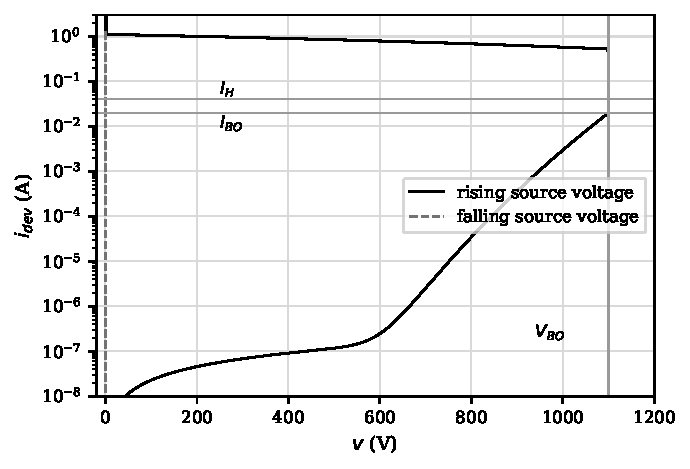
\includegraphics[width=0.72\textwidth]{bod_static_iv}
\caption{Static characteristic of the model (conduction current, logarithmic scale) obtained with a triangular source sweep through \SI{1}{k\ohm}; the vertical segments are the jumps along the load line at breakover and at turn-off.}
\label{fig:static_iv}
\end{figure}

\paragraph{Protection of a thyristor (Fig.~\ref{fig:protection_sim}).} Circuit of Fig.~\ref{fig:protection} with a source ramping at \SI{200}{V\per\micro\second} to \SI{1600}{V} through $R_s=\SI{2}{\ohm}$, $R_1=\SI{150}{\ohm}$, $R_2=\SI{220}{\ohm}$, $C_2=\SI{22}{nF}$, ideal $D_1$, and a functional thyristor with $V_{GT}=\SI{2.5}{V}$, $I_{GT}=\SI{0.3}{A}$, $t_{gd}=\SI{3}{\micro\second}$. The BOD triggers at $t=\SI{5.52}{\micro\second}$ ($v_s=\SI{1104}{V}$, i.e.\ $\Vbo$ plus the drops), the gate current exceeds $I_{GT}$ \SI{25}{ns} later (the collapse of $v_{cl}$ starts immediately), the BOD is fully on after $t_d=\SI{0.3}{\micro\second}$ and carries about \SI{10}{A} (set by $R_1$) until the thyristor turns on at \SI{8.55}{\micro\second}; the anode voltage, which had continued to rise to \SI{1600}{V} during $t_d+t_{gd}$, collapses and the BOD turns off within the same step. The energy dissipated in the BOD is \SI{0.25}{mJ} (\SI{0.2}{mJ} during the \SI{0.3}{\micro\second} collapse, \SI{42}{\micro\joule} in the on-state), against \SI{38}{mJ} in $R_1$.

\begin{figure}[htb]
\centering
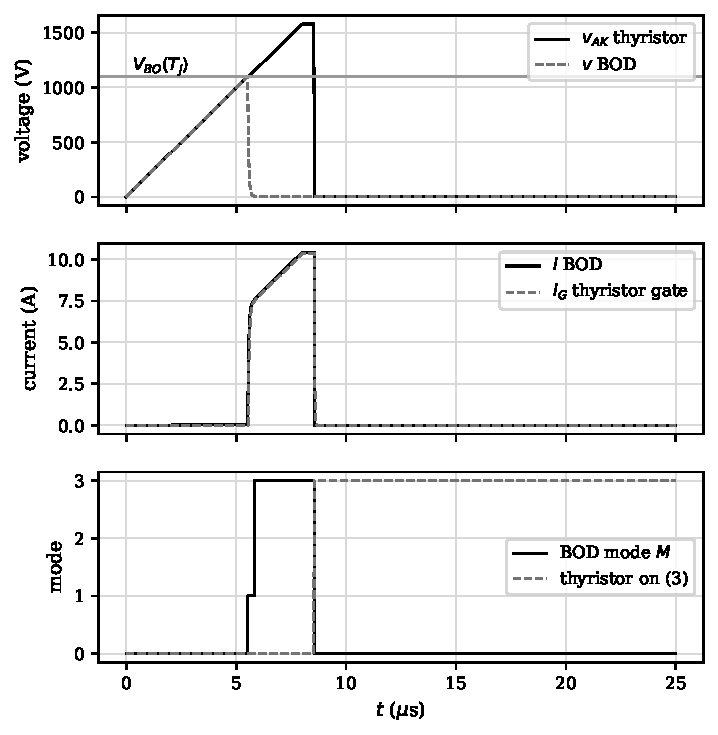
\includegraphics[width=0.8\textwidth]{bod_protection}
\caption{BOD-triggered turn-on of a thyristor (Python replica): anode and BOD voltages, BOD and gate currents, BOD mode and thyristor state.}
\label{fig:protection_sim}
\end{figure}

\paragraph{$\dvdt$ triggering (Fig.~\ref{fig:dvdt}).} Voltage ramps through \SI{10}{\ohm} up to $0.95\,\Vbo$ (\SI{1045}{V}, below $\Vbo$ at both temperatures): \SI{1500}{V\per\micro\second} at \SI{25}{\celsius} does not trigger; \SI{4000}{V\per\micro\second} triggers at \SI{743}{V} $= 0.9\cdot1100\cdot3000/4000$; at \SI{150}{\celsius}, with $(\dvdt)_{cr}=\SI{1000}{V\per\micro\second}$ and $\Vbo=\SI{1238}{V}$, \SI{1500}{V\per\micro\second} triggers at \SI{742}{V}. The voltage then collapses in \SI{0.3}{\micro\second}.

\begin{figure}[htb]
\centering
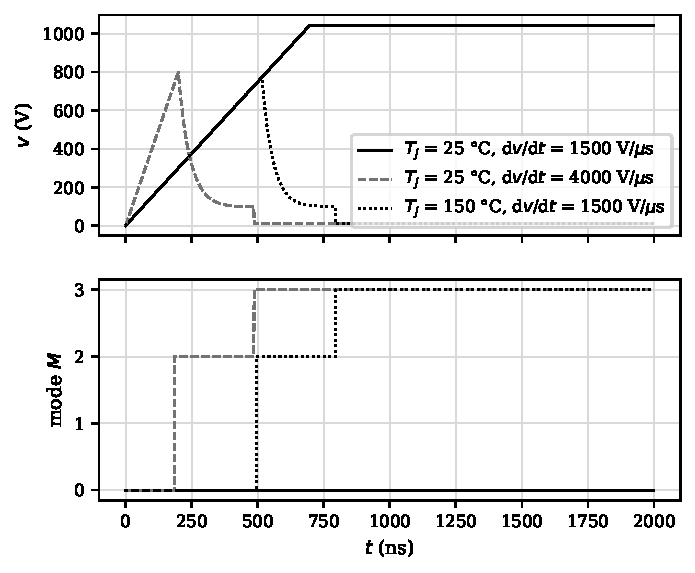
\includegraphics[width=0.72\textwidth]{bod_dvdt}
\caption{$\dvdt$ triggering below $\Vbo$: ramps of 1500 and \SI{4000}{V\per\micro\second} at \SI{25}{\celsius} and \SI{1500}{V\per\micro\second} at \SI{150}{\celsius}, all limited to $0.95\,\Vbo$.}
\label{fig:dvdt}
\end{figure}

\paragraph{Recovery after turn-off (Fig.~\ref{fig:recovery}).} The BOD conducts for \SI{20}{\micro\second} (source \SI{1300}{V} through \SI{20}{\ohm}), the source is removed and a ramp of \SI{200}{V\per\micro\second} is re-applied \SI{50}{\micro\second} or \SI{500}{\micro\second} later. In the first case $x_b=0.71$ and the device re-triggers at $V_{blk}=\SI{797}{V}$; in the second $x_b\approx 1$ and it re-triggers at \SI{1100}{V}.

\begin{figure}[htb]
\centering
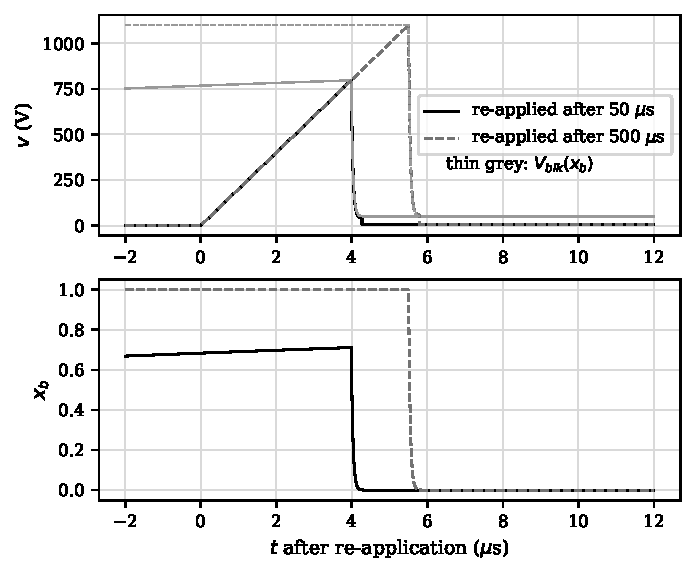
\includegraphics[width=0.72\textwidth]{bod_recovery}
\caption{Re-applied voltage after turn-off: reduced breakover level during the recovery (thin grey line, $V_{blk}(x_b)$) and full $\Vbo$ after more than $2\,t_q$.}
\label{fig:recovery}
\end{figure}

\paragraph{Temperature dependence (Fig.~\ref{fig:temperature}).} $\Vbo$, $\Ih$, $I_D$ and $(\dvdt)_{cr}$ from Eqs.~(\ref{eq:vbot})--(\ref{eq:dvdtt}) between \SI{-40}{\celsius} and \SI{150}{\celsius}, with the datasheet points.

\begin{figure}[htb]
\centering
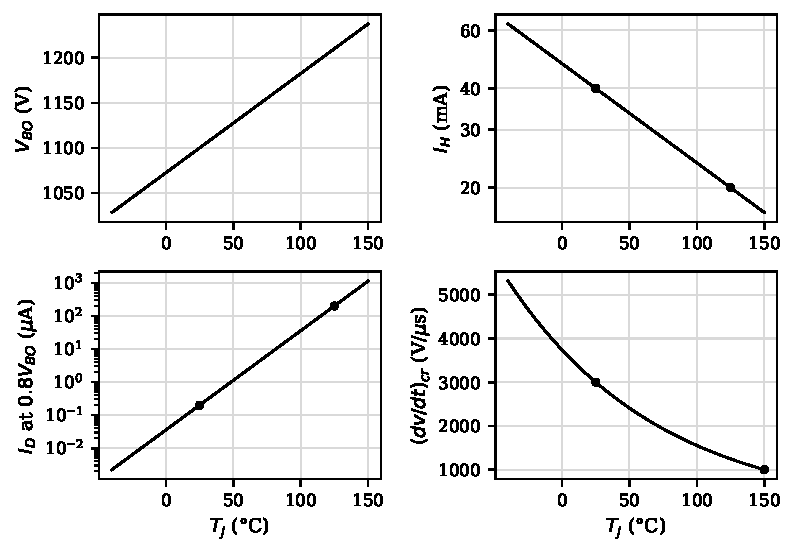
\includegraphics[width=0.78\textwidth]{bod_temperature}
\caption{Temperature dependence used in the model; dots are the datasheet points.}
\label{fig:temperature}
\end{figure}

%======================================================================
\section{Use in the crowbar models}
In the \ssc{+dtt/+crowbar} package the BOD is connected between the anode and the gate node of \ssc{thyristor\_fn} (or of \ssc{thyristor\_rr} in the detailed version) through a Diode block (or \ssc{diode\_fn}) and a resistor $R_1$, as in Fig.~\ref{fig:protection}; the gate node carries the $R_2\parallel C_2$ network and the firing-unit output. For a self-fired crowbar without firing unit the same connection is the only gate source. The output \ssc{M} can be logged or fed to a Scope through a PS-Simulink converter to see whether a firing was caused by voltage ($M=1$) or by $\dvdt$ ($M=2$), which is the diagnostic needed for the spurious firings observed on the machine.

For a stack of $n$ elements one block is used with \ssc{V\_BO}, \ssc{V\_T0}, \ssc{V\_RB}, \ssc{r\_T} and \ssc{r\_av} multiplied by $n$, \ssc{C\_j} divided by $n$, and the parallel sharing resistors added externally. With the thermal port on, a Thermal Mass and a Temperature Source (ambient) connected to H give the junction temperature and, through $K_T$, the drift of the firing level.

Recommended solver settings are those already used for the package: variable-step \ssc{daessc} or \ssc{ode23t}, relative tolerance $10^{-4}$ or tighter, and a maximum step small enough to resolve the \SI{0.3}{\micro\second} collapse when its waveform is of interest.

%======================================================================
\appendix
\section{Listing of \ssc{bod.ssc}}
\label{app:listing}
\begin{lstlisting}[language=Matlab]
component bod
% Break-over diode (BOD)
% Two-terminal p-n-p-n break-over diode used as a passive overvoltage
% trigger for thyristors (anode-to-gate connection).
%
% Functional model with switching dynamics:
%  - forward blocking: temperature-dependent off-state current plus a
%    steep pre-breakover (avalanche-multiplication) term reaching I_BO
%    at the break-over voltage V_BO(T) = V_BO*(1 + K_T*(T - 25 degC));
%  - break-over event at v >= V_BO(T) or by dv/dt (displacement current
%    criterion calibrated at the datasheet point 0.9*V_BO, dv/dt_cr(T));
%  - turn-on: the voltage collapses from V_BO to the on-state along an
%    exponential with total duration t_d (blocking-capability state xb);
%  - on-state: v = V_T0 + r_T*i, turn-off when i < I_H(T);
%  - recovery: after turn-off the blocking capability rebuilds from V_rq
%    to V_BO(T) with the time constant t_q/ln(100) (tq surrogate);
%    a forward voltage re-applied earlier re-triggers the device;
%  - reverse: the BOD blocks only V_RB (about 10 V), beyond that it breaks
%    down with the resistance R_RB (a series diode is required in the
%    application circuit);
%  - junction capacitance C_j in parallel (also provides dv/dt);
%  - optional thermal port H: junction thermal mass C_thj = 1/K_P and
%    junction-to-port resistance R_thjh, dissipation p = v*i_dev.
%
% Output M: 0 blocking, 1 break-over (voltage) triggered, 2 dv/dt
% triggered, 3 on-state.
%
% Default parameters: Littelfuse/IXYS IXBOD2-11 (V_BO = 1100 V +/- 50 V).
% Values marked (assumed) are not given in the datasheet.
%
% Package dtt.crowbar - functional models for the DTT DIV crowbar.
% Rev. 00, 2026-09-22.

nodes
    p = foundation.electrical.electrical; % +:left
    n = foundation.electrical.electrical; % -:right
end

outputs
    M = {0, '1'}; % M:right
end

parameters
    V_BO      = {1100, 'V'};     % Break-over voltage V_BO at 25 degC
    I_BO      = {20,   'mA'};    % Break-over current I_BO
    m_av      = {20,   '1'};     % Exponent of the pre-breakover current
    I_D25     = {0.2,  'uA'};    % Off-state current at 0.8*V_BO, 25 degC
    I_D125    = {200,  'uA'};    % Off-state current at 0.8*V_BO, 125 degC
    V_T0      = {0.9,  'V'};     % On-state threshold voltage V_T0
    r_T       = {80,   'mOhm'};  % On-state slope resistance r_T
    I_H25     = {40,   'mA'};    % Holding current I_H at 25 degC
    I_H125    = {20,   'mA'};    % Holding current I_H at 125 degC
    K_T       = {1e-3, '1/K'};   % Temperature coefficient of V_BO, K_T
    dvdt_cr25 = {3000, 'V/us'};  % Critical dv/dt at 0.9*V_BO, 25 degC
    dvdt_cr150= {1000, 'V/us'};  % Critical dv/dt at 0.9*V_BO, 150 degC
    V_RB      = {10,   'V'};     % Reverse blocking (breakdown) voltage
    R_RB      = {1,    'Ohm'};   % Reverse breakdown resistance (assumed)
    C_j       = {20,   'pF'};    % Junction capacitance (assumed)
    t_d       = {0.3,  'us'};    % Turn-on time, V_BO to on-state (assumed)
    r_av      = {1,    'Ohm'};   % Dynamic resistance during turn-on (assumed)
    t_q       = {200,  'us'};    % Turn-off (recovery) time t_q
    V_rq      = {50,   'V'};     % Blocking capability right after turn-off (assumed)
    T_j       = {25,   'degC'};  % Junction temperature (thermal port off)
    thermal_port = simscape.enum.onoff.off; % Thermal port
    R_thjh    = {60,   'K/W'};   % Thermal resistance junction to port H
    C_thj     = {1.43, 'mJ/K'};  % Junction thermal mass (1/K_P)
end

parameters (Access = private)
    T_ref  = {298.15, 'K'};  % Reference temperature (25 degC)
    T_hot  = {398.15, 'K'};  % Temperature of the I_D125 / I_H125 data (125 degC)
    T_hot2 = {423.15, 'K'};  % Temperature of the dvdt_cr150 data (150 degC)
    x_on   = {1e-3, '1'};    % Blocking-capability level at the end of turn-on
    k_H    = log(I_H25/I_H125)/(T_hot - T_ref);        % I_H decay rate
    k_D    = log(I_D125/I_D25)/(T_hot - T_ref);        % I_D growth rate
    k_dv   = log(dvdt_cr25/dvdt_cr150)/(T_hot2 - T_ref); % dv/dt_cr decay rate
    tau_d  = t_d/log(1/x_on);                          % Turn-on time constant
    tau_q  = t_q/log(100);                             % Recovery time constant (99 % at t_q)
end

variables
    v       = {0, 'V'};    % Voltage
    i       = {0, 'A'};    % Current
    i_dev   = {0, 'A'};    % Conduction current (without C_j)
    dvdt    = {0, 'V/s'};  % dv/dt
    xb      = {value = {1, '1'}, priority = priority.high}; % Blocking capability (0..1)
    V_BOT   = {1100, 'V'}; % Break-over voltage at T_j
    V_blk   = {1100, 'V'}; % Actual blocking capability
    v_cl    = {1100, 'V'}; % Clamp voltage during turn-on
    I_HT    = {40, 'mA'};  % Holding current at T_j
    I_DT    = {0.2, 'uA'}; % Off-state current at T_j
    dvdt_crT= {3000, 'V/us'}; % Critical dv/dt at T_j
    p_d     = {0, 'W'};    % Dissipated power
end

branches
    i : p.i -> n.i;
end

if thermal_port == simscape.enum.onoff.on
    nodes
        H = foundation.thermal.thermal; % H:bottom
    end
    variables
        Tj = {value = {25, 'degC'}, priority = priority.high}; % Junction temperature
        Q  = {0, 'W'}; % Heat flow from port H into the junction
    end
    branches
        Q : H.Q -> *;
    end
    equations
        Q == -(Tj - H.T)/R_thjh;
        C_thj*der(Tj) == p_d + Q;
    end
else
    variables
        Tj = {25, 'degC'}; % Junction temperature
    end
    equations
        Tj == T_j;
    end
end

equations
    assert(C_j > 0, 'The junction capacitance C_j must be positive')
    assert(t_d > 0, 'The turn-on time t_d must be positive')
    assert(t_q > 0, 'The turn-off time t_q must be positive')
    assert(V_rq > V_T0 && V_rq < V_BO, 'V_rq must lie between V_T0 and V_BO')
    assert(V_RB > 0, 'The reverse blocking voltage V_RB must be positive')

    v == p.v - n.v;
    dvdt == der(v);
    i == i_dev + C_j*dvdt;

    % Temperature dependence
    V_BOT    == V_BO*(1 + K_T*(Tj - T_ref));
    I_HT     == I_H25*exp(-k_H*(Tj - T_ref));
    I_DT     == I_D25*exp(k_D*(Tj - T_ref));
    dvdt_crT == dvdt_cr25*exp(-k_dv*(Tj - T_ref));

    % Blocking capability and turn-on clamp
    V_blk == V_rq + xb*(V_BOT - V_rq);
    v_cl  == V_T0 + xb*(V_BOT - V_T0);

    p_d == v*i_dev;
end

modecharts (ExternalAccess = observe)
    bod_mc = modechart
        modes
            mode Blocking
                equations
                    if v >= 0
                        i_dev == I_DT*v/(0.8*V_BOT) + I_BO*(v/V_BOT)^m_av;
                    elseif v >= -V_RB
                        i_dev == I_DT*v/(0.8*V_BOT);
                    else
                        i_dev == I_DT*v/(0.8*V_BOT) + (v + V_RB)/R_RB;
                    end
                    der(xb) == (1 - xb)/tau_q;
                    M == 0;
                end
            end
            mode Triggered
                equations
                    if v > v_cl
                        i_dev == I_DT*v/(0.8*V_BOT) + (v - v_cl)/r_av;
                    else
                        i_dev == I_DT*v/(0.8*V_BOT);
                    end
                    der(xb) == -xb/tau_d;
                    M == 1;
                end
            end
            mode TriggeredDV
                equations
                    if v > v_cl
                        i_dev == I_DT*v/(0.8*V_BOT) + (v - v_cl)/r_av;
                    else
                        i_dev == I_DT*v/(0.8*V_BOT);
                    end
                    der(xb) == -xb/tau_d;
                    M == 2;
                end
            end
            mode On
                equations
                    i_dev == (v - V_T0)/r_T;
                    der(xb) == -xb/tau_d;
                    M == 3;
                end
            end
        end
        transitions
            Blocking    -> Triggered   : v >= V_blk;
            Blocking    -> TriggeredDV : v > 0 && v*dvdt >= 0.9*V_blk*dvdt_crT;
            Triggered   -> On          : xb <= x_on;
            TriggeredDV -> On          : xb <= x_on;
            On          -> Blocking    : i_dev < I_HT;
        end
    end
end

end
\end{lstlisting}

%======================================================================
\begin{thebibliography}{9}
\bibitem{lawatsch1988} H.~Lawatsch and J.~Vitins, ``Protection of thyristors against overvoltage with breakover diodes,'' \emph{IEEE Trans. Ind. Appl.}, vol.~24, no.~3, pp.~444--448, May/June 1988.
\bibitem{ixysapp} IXYS Corporation, ``Breakover diodes -- applications,'' application section of the IXBOD1 data book, 2000.
\bibitem{ixbod2} Littelfuse Inc., ``IXBOD2 breakover diode Gen2 (IXBOD2-07 \ldots IXBOD2-12),'' datasheet, 2026.
\bibitem{ixbod1} Littelfuse Inc. / IXYS, ``IXBOD1 breakover diode Gen1 (IXBOD1-06 \ldots IXBOD1-10),'' datasheet.
\bibitem{ixyspatent} IXYS Corporation, ``Packaged overvoltage protection circuit for triggering thyristors,'' U.S. Patent Application 2014/0332842 A1, Nov. 2014.
\bibitem{baliga} B.~J. Baliga, \emph{Fundamentals of Power Semiconductor Devices}. New York: Springer, 2008, ch.~8 (thyristors).
\bibitem{lutz} J.~Lutz, H.~Schlangenotto, U.~Scheuermann, and R.~De Doncker, \emph{Semiconductor Power Devices: Physics, Characteristics, Reliability}. Berlin: Springer, 2011, ch.~8.
\bibitem{crowbardtt} D.~Bagnara, ``Crowbar for the DTT DIV in-vessel coil power supplies,'' technical note \ssc{crowbar\_dtt\_div.tex}, Rev.~03, and ``Option B configuration,'' \ssc{optionB\_configuration.tex}, Rev.~00, Secom, Sept. 2026.
\bibitem{crowbarself} D.~Bagnara, ``Crowbar thyristor with passive self-firing network,'' technical note \ssc{crowbar\_thyristor\_selftrigger.tex}, Rev.~02, Sept. 2026.
\bibitem{mathworks} The MathWorks, Inc., \emph{Simscape Language Guide}, sections ``Mode Charts'' and ``Conditional Declarations,'' 2026.
\end{thebibliography}

\end{document}
